\documentclass[table,xcolor=pdftex,dvipsnames]{beamer}\usepackage[]{graphicx}\usepackage[]{color}
%% maxwidth is the original width if it is less than linewidth
%% otherwise use linewidth (to make sure the graphics do not exceed the margin)
\makeatletter
\def\maxwidth{ %
  \ifdim\Gin@nat@width>\linewidth
    \linewidth
  \else
    \Gin@nat@width
  \fi
}
\makeatother

\definecolor{fgcolor}{rgb}{0.345, 0.345, 0.345}
\newcommand{\hlnum}[1]{\textcolor[rgb]{0.686,0.059,0.569}{#1}}%
\newcommand{\hlstr}[1]{\textcolor[rgb]{0.192,0.494,0.8}{#1}}%
\newcommand{\hlcom}[1]{\textcolor[rgb]{0.678,0.584,0.686}{\textit{#1}}}%
\newcommand{\hlopt}[1]{\textcolor[rgb]{0,0,0}{#1}}%
\newcommand{\hlstd}[1]{\textcolor[rgb]{0.345,0.345,0.345}{#1}}%
\newcommand{\hlkwa}[1]{\textcolor[rgb]{0.161,0.373,0.58}{\textbf{#1}}}%
\newcommand{\hlkwb}[1]{\textcolor[rgb]{0.69,0.353,0.396}{#1}}%
\newcommand{\hlkwc}[1]{\textcolor[rgb]{0.333,0.667,0.333}{#1}}%
\newcommand{\hlkwd}[1]{\textcolor[rgb]{0.737,0.353,0.396}{\textbf{#1}}}%
\let\hlipl\hlkwb

\usepackage{framed}
\makeatletter
\newenvironment{kframe}{%
 \def\at@end@of@kframe{}%
 \ifinner\ifhmode%
  \def\at@end@of@kframe{\end{minipage}}%
  \begin{minipage}{\columnwidth}%
 \fi\fi%
 \def\FrameCommand##1{\hskip\@totalleftmargin \hskip-\fboxsep
 \colorbox{shadecolor}{##1}\hskip-\fboxsep
     % There is no \\@totalrightmargin, so:
     \hskip-\linewidth \hskip-\@totalleftmargin \hskip\columnwidth}%
 \MakeFramed {\advance\hsize-\width
   \@totalleftmargin\z@ \linewidth\hsize
   \@setminipage}}%
 {\par\unskip\endMakeFramed%
 \at@end@of@kframe}
\makeatother

\definecolor{shadecolor}{rgb}{.97, .97, .97}
\definecolor{messagecolor}{rgb}{0, 0, 0}
\definecolor{warningcolor}{rgb}{1, 0, 1}
\definecolor{errorcolor}{rgb}{1, 0, 0}
\newenvironment{knitrout}{}{} % an empty environment to be redefined in TeX

\usepackage{alltt}
%\documentclass[table,xcolor=pdftex,dvipsnames, handout]{beamer}

%\usepackage{handoutWithNotes}
%\pgfpagesuselayout{4 on 1 with notes}[letterpaper,border shrink=5mm]


\usepackage{beamerthemesplit}
\usepackage[english]{babel}
\usepackage{amsmath}
\usepackage{amssymb}
\usepackage{amsthm}
\usepackage{verbatim}
\usepackage{graphpap}
\usepackage{epic}
\usepackage{pict2e} %To draw line with any slope
\usepackage{color}
\usepackage{natbib}
\usepackage{enumitem}
\usepackage{booktabs}
\usepackage{xcolor}
\usepackage{setspace}
\usepackage{arydshln}
%\usepackage[table]{xcolor}

\bibliographystyle{ajae}

\newcommand{\p}{\partial}

\newcommand {\framedgraphic}[1] {
        \begin{center}
            \includegraphics[width=\textwidth,height=0.7\textheight,keepaspectratio]{#1}
        \end{center}
        \vspace{-1\baselineskip}
}

\usetheme{Boadilla}
\useoutertheme{shadow}
\usecolortheme{beaver}%seagull
\everymath{\color{blue}}
\everydisplay{\color{blue}}

\usefonttheme{professionalfonts}

\usepackage{hyperref}
\hypersetup{
   colorlinks = {true},
   urlcolor = {blue},
   linkcolor = {black},
   citecolor = {black},
   pdfborderstyle={/S/U/W 1},
   urlbordercolor = 0 0 1,
   citebordercolor = 1 1 1,
   filebordercolor = 1 1 1,
   linkbordercolor = 1 1 1,
   pdfauthor = {Sebastien Pouliot}
}

\widowpenalty=10000 % Avoid single line at the end of a page
\clubpenalty=10000  % Avoid single line at the bottom

\title[Biofuels]{Biofuels}
\author[Pouliot]{S\'{e}bastien Pouliot}
\institute{Iowa State University}
\date{Fall 2017}
\IfFileExists{upquote.sty}{\usepackage{upquote}}{}
\begin{document}

%%%%%%%%%%%%%%%%%%%%%%%%%%%%%%%%%%%%%%%%%%%%%%%%%%%%%%%%%%%%%%%%%%%%%%%%%%%%%%%%%%

\begin{frame}
\titlepage
\vspace{-0.4in}
\begin{center}
Lecture notes for Econ 235\\
\end{center}
\end{frame}

%%%%%%%%%%%%%%%%%%%%%%%%%%%%%%%%%%%%%%%%%%%%%%%%%%%%%%%%%%%%%%%%%%%%%%%%%%%%%%%%%%
\section{Introduction}

\begin{frame}{US biofuel policy}
\begin{enumerate}[label=\textbullet]
  \item US biofuel policy is mainly conducted through the Energy programs:
        \begin{enumerate}[label=-]
          \item Energy Policy Act of 2005 first established Renewable Fuel Standards (RFS); which were quickly surpassed.
          \item The Energy Independence and Security Act of 2007 expanded the RFS and included mandates for advanced biofuels.
          \item The RFS under the Energy Independence and Security Act of 2007 are referred to as RFS2.
      \end{enumerate}
  \item Recent farm bills (Farm Security Act of 2002 and the Food, Conservation, and Energy Act of 2008) also play a role in biofuel policies.
\end{enumerate}
\end{frame}

%%%%%%%%%%%%%%%%%%%%%%%%%%%%%%%%%%%%%%%%%%%%%%%%%%%%%%%%%%%%%%%%%%%%%%%%%%%%%%%%%%

\begin{frame}{References}
\begin{enumerate}[label=\textbullet]
    \item Renewable Fuel Standards (RFS): Overview and Issues \url{http://www.fas.org/sgp/crs/misc/R40155.pdf}.
    \item Biofuel Incentives: A Summary of Federal Programs \url{http://www.fas.org/sgp/crs/misc/R40110.pdf}.
    \item The Renewable Fuel Standard (RFS): In Brief \url{http://nationalaglawcenter.org/wp-content/uploads/assets/crs/R43325.pdf}.
\end{enumerate}
\end{frame}

%%%%%%%%%%%%%%%%%%%%%%%%%%%%%%%%%%%%%%%%%%%%%%%%%%%%%%%%%%%%%%%%%%%%%%%%%%%%%%%%%%

\begin{frame}{Definitions}
\begin{enumerate}[label=\textbullet]
    \item \emph{Advanced biofuels} are produced from non-corn starch feedstocks. These biofuels must also meet certain minimum thresholds of lifecycle greenhouse gas emission reduction to qualify as advanced biofuels.
    \item These notes focus mostly on ethanol produced from corn.
    \item In biofuel policy, a \emph{mandate} defines the minimum quantity of a biofuel that must be blended into motor fuel.
\end{enumerate}
\end{frame}

%%%%%%%%%%%%%%%%%%%%%%%%%%%%%%%%%%%%%%%%%%%%%%%%%%%%%%%%%%%%%%%%%%%%%%%%%%%%%%%%%%

\begin{frame}{Renewable Fuel Requirements (RFS2) in billion gallons}
\tiny
\begin{center}
\rowcolors{10}{gray!35}{gray!35}
\begin{tabular}{ccccccc}
  \toprule
  & & \multicolumn{4}{c}{Advanced biofuels} & \\
  \cmidrule(r){3-6}
  Year & \parbox[b]{0.70in}{\centering Corn starch ethanol} & \parbox[b]{0.50in}{\centering Cellulosic} & \parbox[b]{0.50in}{\centering Bio-based diesel} & \parbox[b]{0.5in}{\centering Other} & \parbox[b]{0.5in}{\centering Total non-corn starch} & \parbox[b]{0.55in}{\centering Total renewable fuels} \\
  \midrule
  2008 & 9.0  & 0.00     & 0.00 & 0.00 & 0.00 & 9.0 \\
  2009 & 10.5 & 0.00     & 0.00 & 0.10 & 0.60 & 11.1 \\
  2010 & 12.0 & 0.0065 & 1.15 & 0.29 & 0.95 & 12.95 \\
  2011 & 12.6 & 0.006  & 0.80 & 0.54 & 1.35 & 13.95 \\
  2012 & 13.2 & 0.00   & 1.00 & 1.00 & 2.00 & 15.20 \\
  2013 & 13.8 & 0.014  & 1.28 & 1.46 & 2.75 & 16.55 \\
  2014 & 14.4 & 1.75   & a    & 1.00 & 3.75 & 18.15 \\
  2015 & 15.0 & 3.00   & a    & 1.50 & 5.50 & 20.50 \\
  2016 & 15.0 & 4.25   & a    & 2.00 & 7.25 & 22.25 \\
  \hdashline
  2017 & 15.0 & 5.50   & a    & 2.50 & 9.00 & 24.00 \\
  2018 & 15.0 & 7.00   & a    & 3.00 & 11.00 & 26.00 \\
  2019 & 15.0 & 8.50   & a    & 3.50 & 13.00 & 28.00 \\
  2020 & 15.0 & 10.50  & a    & 3.50 & 15.00 & 30.00 \\
  2021 & 15.0 & 13.50  & a    & 3.50 & 18.00 & 33.00 \\
  2022 & 15.0 & 16.00  & a    & 4.00 & 21.00 & 36.00 \\
  2023 & 15.0 & b      & b    & b    & b     & b \\
  \bottomrule
\end{tabular}
\end{center}
\singlespace
Notes: Before 2014 the numbers are the actual biofuel mandates. After 2014, the numbers are the volumes that were planned in the RFS.

The source of the table is \cite{Schnepf2013}. \emph{na} stands for ``non-applicable" and \emph{tbd} stands for ``to be determined". a. means to be determined by EPA but no less than one billion gallon. b. means to be determined by EPA through future rulemaking.
\end{frame}

%%%%%%%%%%%%%%%%%%%%%%%%%%%%%%%%%%%%%%%%%%%%%%%%%%%%%%%%%%%%%%%%%%%%%%%%%%%%%%%%%%

\begin{frame}{Renewable Fuel Requirements (RFS2) in billion gallons}\label{slide.mandates}
\begin{enumerate}[label=\textbullet]
    \item There was a lot of controversy about the biofuel volumes for 2014.
    \item The final volumes for 2014 were only released in June 2015.
    \item At the same time EPA also released volumes for 2015 and 2016.
    \item We will discuss this more at the end of this section.
\end{enumerate}
\tiny
\begin{table}
\begin{center}
\caption{Biofuel volumes for 2014-17}
\begin{tabular}{ccccccc}
  \toprule
  & & \multicolumn{4}{c}{Advanced biofuels} & \\
  \cmidrule(r){3-6}
  Year & \parbox[b]{0.70in}{\centering Corn starch ethanol} & \parbox[b]{0.50in}{\centering Cellulosic} & \parbox[b]{0.50in}{\centering Bio-based diesel} & \parbox[b]{0.5in}{\centering Other} & \parbox[b]{0.5in}{\centering Total non-corn starch} & \parbox[b]{0.55in}{\centering Total renewable fuels} \\
  \midrule
  2014 & 13.61 & 0.03   & 1.63    & 1.01 & 2.67 & 16.28 \\
  2015 & 14.05 & 0.12   & 1.73    & 1.03 & 2.88 & 16.93 \\
  2016 & 14.50 & 0.23   & 1.90    & 1.48 & 3.61 & 18.11 \\
  2017 & 15.00 & 0.31   & 2.00    & 1.69 & 4.28 & 19.28 \\
  \bottomrule
\end{tabular}
\end{center}
\end{table}
\singlespace
Source: \url{https://www.epa.gov/renewable-fuel-standard-program/proposed-renewable-fuel-standards-2017-and-biomass-based-diesel}.
\end{frame}

%%%%%%%%%%%%%%%%%%%%%%%%%%%%%%%%%%%%%%%%%%%%%%%%%%%%%%%%%%%%%%%%%%%%%%%%%%%%%%%%%%

\begin{frame}{Tax credits and tariffs}
\begin{enumerate}[label=\textbullet]
    \item Volumetric Ethanol Excise Tax Credit (VEETC): Ethanol blenders were eligible for a 51 cents per gallon of ethanol tax credit. The 2008 farm bill amended the tax credit which was 45 cents per gallon between January 2009 and December 31, 2011. This credit is now expired.
    \item An import tariff of 54 cents per gallon for ethanol. The import tariff was set to offset the tax credit, thus effectively cancelling the tax credit for imported ethanol. As long as the import tariff is larger that the blending tax credit, on the net, imports are taxed. The import tariff expired on December 31, 2011.
\end{enumerate}
\end{frame}


%%%%%%%%%%%%%%%%%%%%%%%%%%%%%%%%%%%%%%%%%%%%%%%%%%%%%%%%%%%%%%%%%%%%%%%%%%%%%%%%%%

\begin{frame}{Who the mandates apply to?}
\begin{enumerate}[label=\textbullet]
    \item The implementation of RFS2 is done through annual requirements set by the Environmental Protection Agency (EPA) based on projections on the consumption of gasoline and diesel from the Energy Information Administration (EIA).
    \item Each November, EPA sets the percentage of fuel by category that must come from renewable sources in the following year.
    \item EPA sets those percentages using demand estimates and production capacity estimates. Note that EPA can, through rulemaking, modify the mandated quantities if the infrastructure to produce biofuel quantities does not exist.
    \item Gasoline refiners are obligated to obtain credit for a quantity of biofuel equal to a percentage of their total annual fuel sales, for each of the four biofuel categories. This requirement is referred to as the Renewable Volume Obligation (RVO).
\end{enumerate}
\end{frame}

%%%%%%%%%%%%%%%%%%%%%%%%%%%%%%%%%%%%%%%%%%%%%%%%%%%%%%%%%%%%%%%%%%%%%%%%%%%%%%%%%%

\section{Impact of biofuel on farms}

\begin{frame}{How does the ethanol policy affect farms}
\begin{enumerate}[label=\textbullet]
    \item It works in a way similar to pollution permits.
    \item To meet their RVO, refiners purchase a RIN from fuel blenders which is then submitted to EPA to show compliance with the RVO.
    \item A RIN shows that one gallon of ethanol has been blended in gasoline.
    \item Thus, as refiners demand RINs, blenders will demand ethanol to be able to sell RINs to refiners.
    \item As most ethanol is produced from corn in the United States, the increase in the demand for ethanol increases the demand for corn.
    \item The increase in the demand for corn causes the price and the quantity of corn to increase.
\end{enumerate}
\end{frame}


%%%%%%%%%%%%%%%%%%%%%%%%%%%%%%%%%%%%%%%%%%%%%%%%%%%%%%%%%%%%%%%%%%%%%%%%%%%%%%%%%%

\begin{frame}{RIN and ethanol markets diagram}
    \framedgraphic{Model_RIN.png}
\end{frame}

%%%%%%%%%%%%%%%%%%%%%%%%%%%%%%%%%%%%%%%%%%%%%%%%%%%%%%%%%%%%%%%%%%%%%%%%%%%%%%%%%%

\begin{frame}{Shifts in demand for corn}
\begin{figure}[htbp]
\begin{center}
    \begin{picture}(240,180)
        %Axises and labels
        \scriptsize
        \put(0,0){\vector(1,0){240}} %x-axis
        \put(0,0){\vector(0,1){180}} %y-axis
        \put(225,-10){$Q$}
        \put(-5,170){\makebox(0,0){$P$}}
        %Demand curve
        \thicklines
        \put(0,140){\line(1,-1){140}}
        %Supply curve
        \put(0,0){\line(1,1){160}}
        %Text
        \put(135,10){$D_0$}
        \put(150,155){$S$}
        %Equilibrium
        \color{black}
        \multiput(0,70)(5,0){14}{\line(1,0){2.5}}%Dashed line
        \multiput(70,70)(0,-5){14}{\line(0,-1){2.5}}%Dashed line
        \put(-10,68){$P_0$}
        \put(68,-10){$Q_0$}
        \onslide<1>{
        \put(50,150){Before mandate}}
        %Positive shift in demand
        \onslide<2>
        \put(50,150){With mandate}
        \color{blue}
        \put(0,160){\line(1,-1){160}}
        \put(40,100){\vector(1,0){20}} %x-axis
        \put(155,10){$D_1$}
        \multiput(0,80)(5,0){16}{\line(1,0){2.5}}%Dashed line h
        \multiput(80,80)(0,-5){16}{\line(0,-1){2.5}}%Dashed line v
        \put(78,-10){$Q_1$}
        \put(-10,78){$P_1$}
    \end{picture}
\vspace{0.1in}
\end{center}
\end{figure}
\end{frame}



%%%%%%%%%%%%%%%%%%%%%%%%%%%%%%%%%%%%%%%%%%%%%%%%%%%%%%%%%%%%%%%%%%%%%%%%%%%%%%%%%%

\begin{frame}{Were mandates really the reason for the growth of the ethanol industry?}
\begin{enumerate}[label=\textbullet]
    \item At the same time as EPA instituted the first ethanol mandates, Congress removed oxygenate requirements (which raises octane number) for gasoline.
    \item In response, refiners stopped using Methyl Tertiary Butyl Ether (MTBE) and instead started using ethanol to increase octane in gasoline.
    \item This means that refiners would use a certain amount of ethanol whether the ethanol mandates were in place or not.
    \item As ethanol is a substitute to gasoline, blenders would even use as much ethanol as possible in motor fuel if it is cheaper than gasoline.
    \item This means that blenders might use more ethanol then the mandated volume.
    \item Whether the growth of US ethanol industry is entirely attributable to the ethanol mandates is debatable.
\end{enumerate}
\end{frame}

%http://www.epa.gov/mtbe/gas.htm

%%%%%%%%%%%%%%%%%%%%%%%%%%%%%%%%%%%%%%%%%%%%%%%%%%%%%%%%%%%%%%%%%%%%%%%%%%%%%%%%%%



\begin{frame}{Price for corn, wholesale ethanol and wholesale gasoline}
\begin{knitrout}
\definecolor{shadecolor}{rgb}{0.969, 0.969, 0.969}\color{fgcolor}
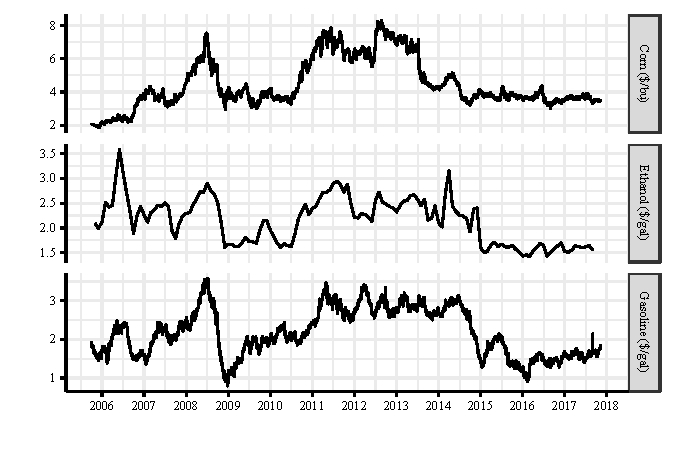
\includegraphics[width=\maxwidth]{figure/figure_price-1} 

\end{knitrout}
\vspace{-1\baselineskip}
\scriptsize
Sources: Prices for corn and gasoline are the daily settle prices of the nearest expiring futures contracts. The price of ethanol is the monthly F.O.B. ethanol rack price in Omaha, Nebraska given at \url{http://www.neo.ne.gov/statshtml/66.html}.
\end{frame}

%%%%%%%%%%%%%%%%%%%%%%%%%%%%%%%%%%%%%%%%%%%%%%%%%%%%%%%%%%%%%%%%%%%%%%%%%%%%%%%%%%

\begin{frame}{Mandate vs production and consumption}
\begin{enumerate}[label=\textbullet]
    \item After the adoption of the first mandates (RFS1), the industry quickly outpaced the ethanol mandate.
    \item RFS2 increased the biofuel mandates but still refiners blended more ethanol than what was required by the mandates until 2012.
    \item Early on, the US was a net importer of ethanol and then became an net exporter of ethanol.
\end{enumerate}
\end{frame}

%%%%%%%%%%%%%%%%%%%%%%%%%%%%%%%%%%%%%%%%%%%%%%%%%%%%%%%%%%%%%%%%%%%%%%%%%%%%%%%%%%

\begin{frame}{Mandate vs production and consumption (up to May 2017)}
\begin{knitrout}
\definecolor{shadecolor}{rgb}{0.969, 0.969, 0.969}\color{fgcolor}
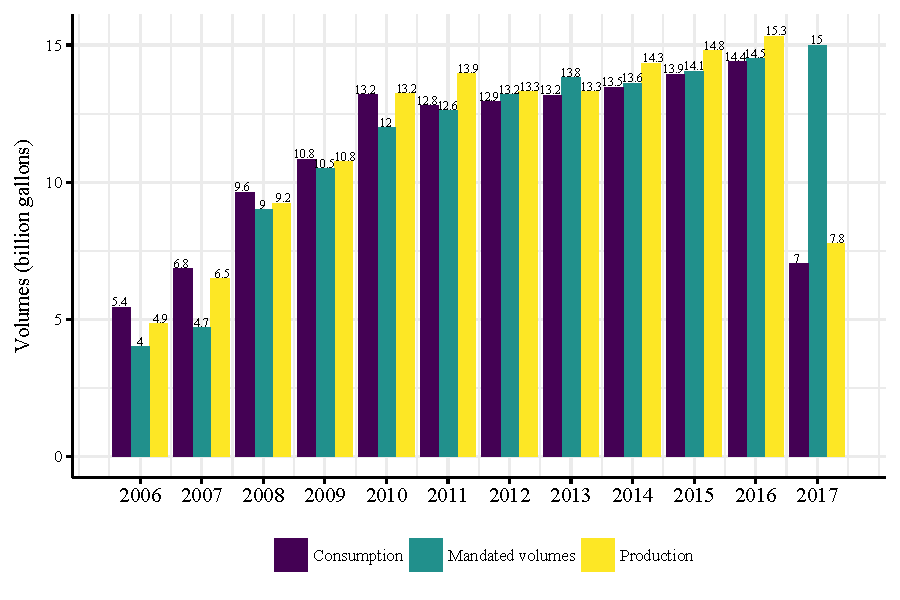
\includegraphics[width=\maxwidth]{figure/figure_rfs2-1} 

\end{knitrout}
\end{frame}


%%%%%%%%%%%%%%%%%%%%%%%%%%%%%%%%%%%%%%%%%%%%%%%%%%%%%%%%%%%%%%%%%%%%%%%%%%%%%%%%%%

\section{Return to ethanol production}


\begin{frame}{Profit of producing ethanol}
\begin{enumerate}[label=\textbullet]
    \item Let's look at what affects the profitability of ethanol plants.
    \item Several websites offer measures of profitability:
    \begin{enumerate}[label=-]
        \item CARD: \url{http://www.card.iastate.edu/research/biorenewables/tools/hist_eth_gm.aspx};
        \item ISU extension: \url{https://www.extension.iastate.edu/agdm/decisionaidsall.html}.
    \end{enumerate}
    \item We will calculate profits by an ethanol plant using the assumptions of ISU extension, with the excel sheet available \href{https://www.extension.iastate.edu/agdm/energy/xls/d1-10ethanolprofitability.xlsx}{here}.
    \item This gives a good idea of the profit of a representative ethanol plant.
\end{enumerate}
\end{frame}

%http://www.agmrc.org/renewable_energy/

%%%%%%%%%%%%%%%%%%%%%%%%%%%%%%%%%%%%%%%%%%%%%%%%%%%%%%%%%%%%%%%%%%%%%%%%%%%%%%%%%%


\begin{frame}{Profit of producing ethanol}
\begin{enumerate}[label=\textbullet]
    \item The excel sheet clearly states the main assumptions to calculate profitability by an ethanol plant:
    \begin{enumerate}[label=-]
        \item Built in 2007;
        \item Capacity of 100 million gallons;
        \item ...
    \end{enumerate}
    \item We will look at the profitability of such a plant located in Iowa.
\end{enumerate}
\end{frame}

%%%%%%%%%%%%%%%%%%%%%%%%%%%%%%%%%%%%%%%%%%%%%%%%%%%%%%%%%%%%%%%%%%%%%%%%%%%%%%%%%%

\begin{frame}{Revenue of ethanol plants}
\begin{enumerate}[label=\textbullet]
    \item A typical corn ethanol plant gets revenue by the production of three outputs:
    \begin{enumerate}[label=-]
        \item Ethanol;
        \item Dried Distillers Grains with Solubles (DDGS);
        \item Corn oil.
    \end{enumerate}
    \item DDGS is a by-product of the production of ethanol. It is a closed substitute to corn as a feed and as such its price follows the price of corn.
    \item I do not have data about corn oil and will ignore its impact on revenue in what follows. It has become a small but significant part of ethanol plant total revenue.
\end{enumerate}
\end{frame}

%http://www.agmrc.org/renewable_energy/

%%%%%%%%%%%%%%%%%%%%%%%%%%%%%%%%%%%%%%%%%%%%%%%%%%%%%%%%%%%%%%%%%%%%%%%%%%%%%%%%%%

\begin{frame}{Prices for corn and DDGS}
\begin{knitrout}
\definecolor{shadecolor}{rgb}{0.969, 0.969, 0.969}\color{fgcolor}
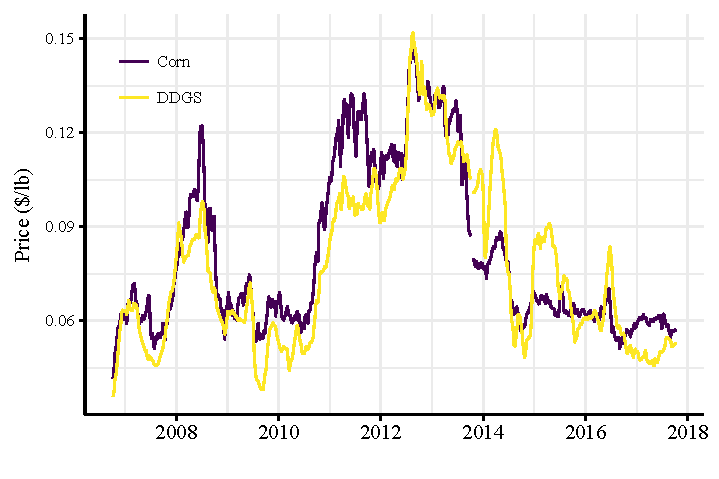
\includegraphics[width=\maxwidth]{figure/figure_ddgs-1} 

\end{knitrout}
\vspace{-1\baselineskip}
Sources: Price data were obtained from \href{http://www.extension.iastate.edu/agdm/energy/xls/agmrcethanolplantprices.xlsx}{AgMRC}.
\end{frame}

%%%%%%%%%%%%%%%%%%%%%%%%%%%%%%%%%%%%%%%%%%%%%%%%%%%%%%%%%%%%%%%%%%%%%%%%%%%%%%%%%%

\begin{frame}{Revenue of ethanol plants}
\begin{enumerate}[label=\textbullet]
    \item One bushel of corn yields about 2.8 gallons of ethanol.
    \item One bushel of corn yields about 16.5 pounds of DDGS.
    \item This is means that for each gallon of ethanol produced, the ethanol plant produces 5.9 pounds of DDGS.
    \item For a price of ethanol of \$2.10 per gallon and a price of DDGS of \$0.10 per pound, the revenues of an ethanol plant for the production of one gallon ethanol are:
    \begin{enumerate}[label=-]
        \item \$2.10 for ethanol;
        \item \$0.59 for the production of DDGS;
        \item Thus a total revenue of \$2.69 for the production of one gallon of ethanol.
    \end{enumerate}
\end{enumerate}
\end{frame}

%%%%%%%%%%%%%%%%%%%%%%%%%%%%%%%%%%%%%%%%%%%%%%%%%%%%%%%%%%%%%%%%%%%%%%%%%%%%%%%%%%

\begin{frame}{Ethanol plants revenues from corn and DDGS}
\begin{knitrout}
\definecolor{shadecolor}{rgb}{0.969, 0.969, 0.969}\color{fgcolor}
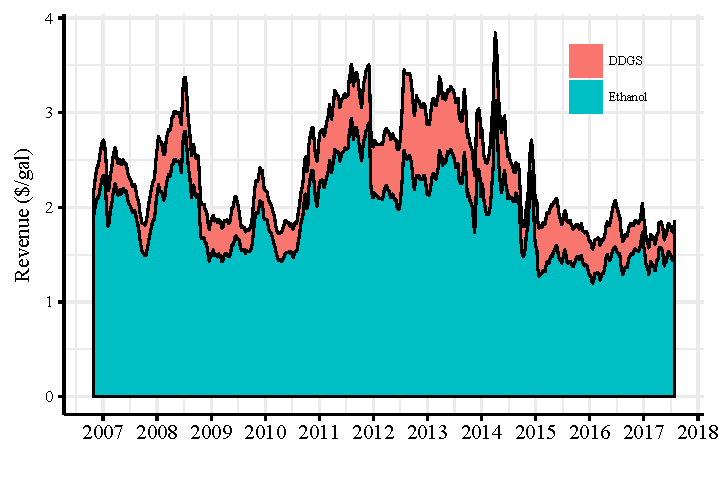
\includegraphics[width=\maxwidth]{figure/figure_rev2-1} 

\end{knitrout}
\vspace{-1\baselineskip}
\scriptsize
Calculations done using price data from \href{http://www.extension.iastate.edu/agdm/energy/xls/agmrcethanolplantprices.xlsx}{AgMRC}.
\end{frame}


%%%%%%%%%%%%%%%%%%%%%%%%%%%%%%%%%%%%%%%%%%%%%%%%%%%%%%%%%%%%%%%%%%%%%%%%%%%%%%%%%%

\begin{frame}{Ethanol plants revenues from corn and DDGS}
\begin{knitrout}
\definecolor{shadecolor}{rgb}{0.969, 0.969, 0.969}\color{fgcolor}
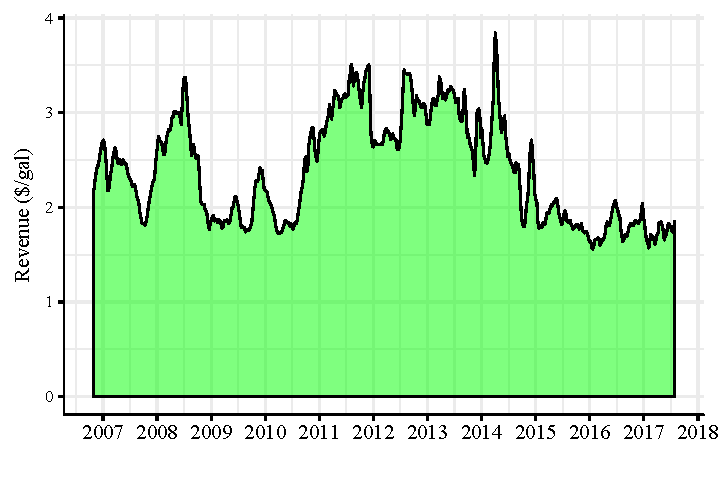
\includegraphics[width=\maxwidth]{figure/figure_rev-1} 

\end{knitrout}
\vspace{-1\baselineskip}
\scriptsize
This is the same graph as on the previous slide but removing detail of the source of revenues.\\
Calculations done using price data from \href{http://www.extension.iastate.edu/agdm/energy/xls/agmrcethanolplantprices.xlsx}{AgMRC}.
\end{frame}

%%%%%%%%%%%%%%%%%%%%%%%%%%%%%%%%%%%%%%%%%%%%%%%%%%%%%%%%%%%%%%%%%%%%%%%%%%%%%%%%%%

\begin{frame}{Cost of ethanol plants}
\begin{enumerate}[label=\textbullet]
    \item A small share of the costs to an ethanol plant is relatively constant and predictable:
    \begin{enumerate}[label=-]
        \item Chemicals: enzymes, yeasts, chemicals and denaturants;
        \item Other direct costs: repair \& maintenance, transportation, water, electricity,...;
        \item Fixed cost: Depreciation, interest, labor \& management and property taxes.
    \end{enumerate}
    \item I would not put labor \& management in the fixed cost category as the excel sheet does but let's leave it there for this exercise.
\end{enumerate}
\end{frame}

%%%%%%%%%%%%%%%%%%%%%%%%%%%%%%%%%%%%%%%%%%%%%%%%%%%%%%%%%%%%%%%%%%%%%%%%%%%%%%%%%%

\begin{frame}{Cost of ethanol plants}
\begin{enumerate}[label=\textbullet]
    \item The largest share of the costs to an ethanol plant are from corn and natural gas.
    \item The prices of these inputs, especially corn, are highly volatile.
\end{enumerate}
\end{frame}


%%%%%%%%%%%%%%%%%%%%%%%%%%%%%%%%%%%%%%%%%%%%%%%%%%%%%%%%%%%%%%%%%%%%%%%%%%%%%%%%%%

\begin{frame}{Ethanol plants costs from corn and DDGS}
\begin{knitrout}
\definecolor{shadecolor}{rgb}{0.969, 0.969, 0.969}\color{fgcolor}
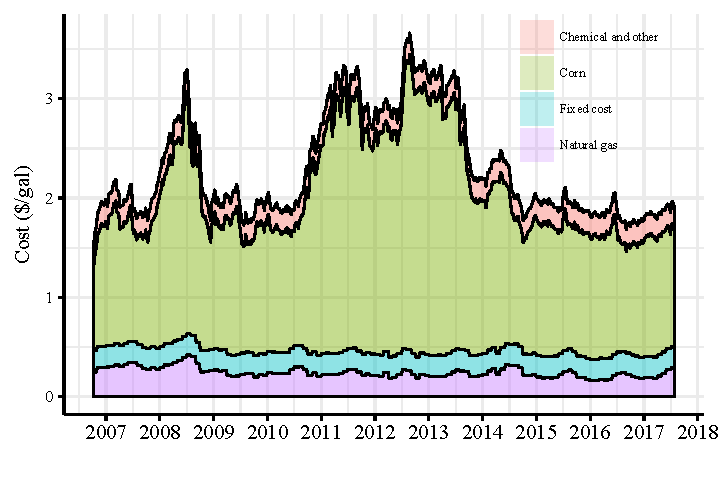
\includegraphics[width=\maxwidth]{figure/figure_cost-1} 

\end{knitrout}
\vspace{-1\baselineskip}
\scriptsize
Calculations done using price data from \href{http://www.extension.iastate.edu/agdm/energy/xls/agmrcethanolplantprices.xlsx}{AgMRC} and from \href{http://www.eia.gov/dnav/ng/ng_pri_sum_dcu_sia_m.htm}{EIA}.
\end{frame}

%%%%%%%%%%%%%%%%%%%%%%%%%%%%%%%%%%%%%%%%%%%%%%%%%%%%%%%%%%%%%%%%%%%%%%%%%%%%%%%%%%

\begin{frame}{Ethanol plants costs from corn and DDGS}
\begin{knitrout}
\definecolor{shadecolor}{rgb}{0.969, 0.969, 0.969}\color{fgcolor}
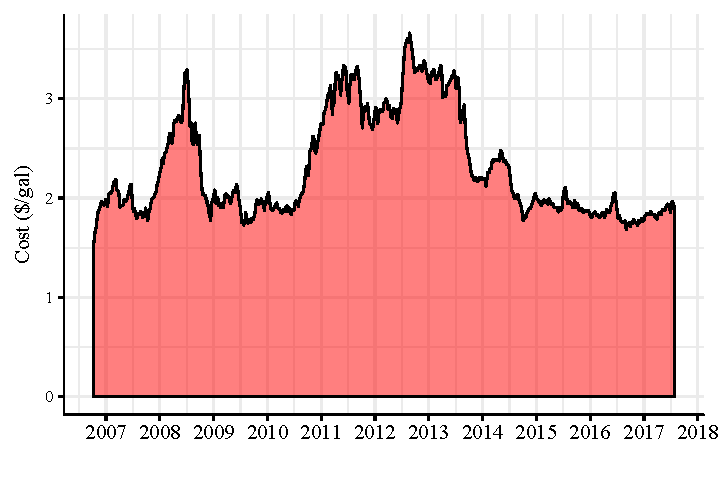
\includegraphics[width=\maxwidth]{figure/figure_cost2-1} 

\end{knitrout}
\vspace{-1\baselineskip}
\scriptsize
This is the same graph as on the previous slide but removing detail of the source of costs.\\
Calculations done using price data from \href{http://www.extension.iastate.edu/agdm/energy/xls/agmrcethanolplantprices.xlsx}{AgMRC} and from \href{http://www.eia.gov/dnav/ng/ng_pri_sum_dcu_sia_m.htm}{EIA}.
\end{frame}

%%%%%%%%%%%%%%%%%%%%%%%%%%%%%%%%%%%%%%%%%%%%%%%%%%%%%%%%%%%%%%%%%%%%%%%%%%%%%%%%%%

\begin{frame}{Profit of ethanol plants}
\begin{enumerate}[label=\textbullet]
    \item We can now calculate the profit of a plant as simply the difference between revenue and the cost.
    \item Note that it likely underestimate profit because revenue from corn oil are not added.
\end{enumerate}
\end{frame}

%%%%%%%%%%%%%%%%%%%%%%%%%%%%%%%%%%%%%%%%%%%%%%%%%%%%%%%%%%%%%%%%%%%%%%%%%%%%%%%%%%

\begin{frame}{Profit of ethanol plant}
\begin{knitrout}
\definecolor{shadecolor}{rgb}{0.969, 0.969, 0.969}\color{fgcolor}
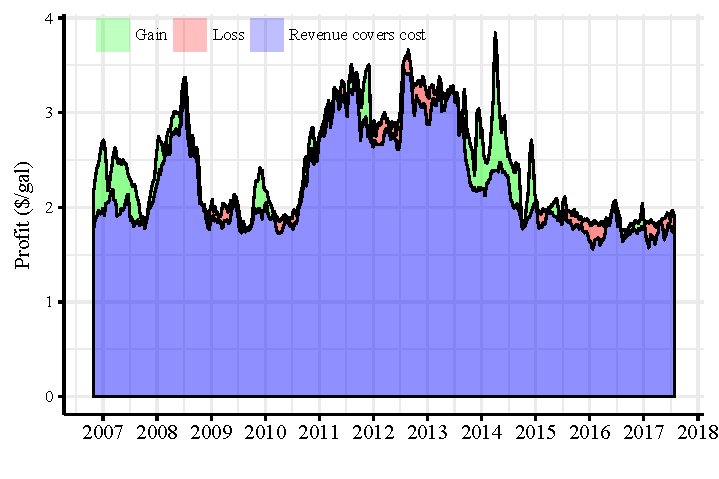
\includegraphics[width=\maxwidth]{figure/figure_pi-1} 

\end{knitrout}
\end{frame}

%%%%%%%%%%%%%%%%%%%%%%%%%%%%%%%%%%%%%%%%%%%%%%%%%%%%%%%%%%%%%%%%%%%%%%%%%%%%%%%%%%

\begin{frame}{Profit of ethanol plant}
\begin{knitrout}
\definecolor{shadecolor}{rgb}{0.969, 0.969, 0.969}\color{fgcolor}
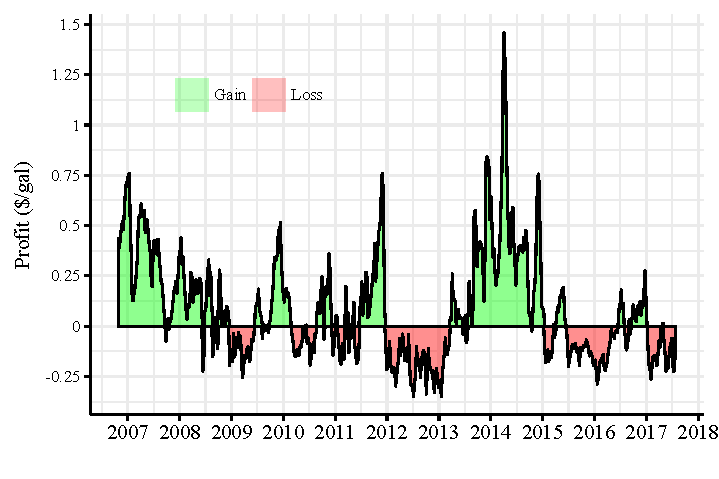
\includegraphics[width=\maxwidth]{figure/figure_pi2-1} 

\end{knitrout}
\end{frame}


%%%%%%%%%%%%%%%%%%%%%%%%%%%%%%%%%%%%%%%%%%%%%%%%%%%%%%%%%%%%%%%%%%%%%%%%%%%%%%%%%%

\begin{frame}{Profit of ethanol plant: corn and ethanol prices}
    \framedgraphic{3_graphs.png}
\end{frame}


%%%%%%%%%%%%%%%%%%%%%%%%%%%%%%%%%%%%%%%%%%%%%%%%%%%%%%%%%%%%%%%%%%%%%%%%%%%%%%%%%%

\begin{frame}{Profit of ethanol plants - volatility}
\begin{enumerate}[label=\textbullet]
    \item The previous figure shows that the profit of an ethanol plant is highly volatile.
    \item The calculation of the profit of a representative ethanol plant assumes that the plant does not hedge.
    \item A plant that hedges on the corn and the ethanol market will have much less volatile profits.
\end{enumerate}
\end{frame}

%%%%%%%%%%%%%%%%%%%%%%%%%%%%%%%%%%%%%%%%%%%%%%%%%%%%%%%%%%%%%%%%%%%%%%%%%%%%%%%%%%

\section{Enforcing the ethanol mandate: RIN}

\begin{frame}{Renewable Identification Numbers (RIN)}
\begin{enumerate}[label=\textbullet]
    \item A RIN is a 38-character number that is attached to one gallon of ethanol produced or imported in the United States.
    \item The RINs remain ``attached" to biofuels until the biofuel has been blended or sold.
    \item After being detached, RINs are tradeable and then effectively become a commodity available for purchase by refiners.
    \item A RIN is valid in the current and the following year.
    \item The objective of RINs is to enforce biofuel mandates and minimize the cost of meeting the mandate.
    \item At the end of the year, each supplier must have enough RINs to show compliance with their RVO.
      \begin{enumerate}[label=-]
          \item This means that a supplier may never sell any biofuel but still meet its RVO through the purchase of RINs.
      \end{enumerate}
\end{enumerate}
\end{frame}

%%%%%%%%%%%%%%%%%%%%%%%%%%%%%%%%%%%%%%%%%%%%%%%%%%%%%%%%%%%%%%%%%%%%%%%%%%%%%%%%%%

\begin{frame}{RIN and ethanol markets diagram}
    \framedgraphic{Model_RIN.png}
\end{frame}

%%%%%%%%%%%%%%%%%%%%%%%%%%%%%%%%%%%%%%%%%%%%%%%%%%%%%%%%%%%%%%%%%%%%%%%%%%%%%%%%%%

\begin{frame}{Renewable Identification Numbers (RIN)}
\begin{enumerate}[label=\textbullet]
    \item RINs differ depending on the type of biofuel they apply to:
      \begin{enumerate}[label=-]
          \item Conventional ethanol RIN (D6);
          \item Advanced ethanol RIN (D5);
          \item Biodiesel RIN (D4);
          \item Cellulosic RIN (D3).
      \end{enumerate}
    \item D\# identifies the type of biofuel within the RIN 38-character number.
    \item The RINs of some biofuels are worth more.
    \item RIN for one type of biofuel qualifies for the type of biofuel above it (see next figure).
      \begin{enumerate}[label=-]
          \item A D5 RIN can be used as a D6 RIN; same with other RIN types.
          \item This creates an ordering in RIN prices.
      \end{enumerate}
\end{enumerate}
\end{frame}

%%%%%%%%%%%%%%%%%%%%%%%%%%%%%%%%%%%%%%%%%%%%%%%%%%%%%%%%%%%%%%%%%%%%%%%%%%%%%%%%%%

\begin{frame}{Nested RFS and RINs}
    \framedgraphic{Nested_RFS.png}
\scriptsize
Source: Analysis of Renewable Identification Numbers (RINs) in the Renewable Fuel Standard (RFS) \url{http://www.hsdl.org/?abstract&did=726857}.
\end{frame}

%%%%%%%%%%%%%%%%%%%%%%%%%%%%%%%%%%%%%%%%%%%%%%%%%%%%%%%%%%%%%%%%%%%%%%%%%%%%%%%%%%

\begin{frame}{The price of RINs}
\begin{enumerate}[label=\textbullet]
    \item The price of RINs is determined by the vertical distance between the supply of ethanol and the demand for ethanol at a given mandated volume.
    \item If the mandate ($Q^M$ in the next figure) is below the market equilibrium, then the price of RIN equals zero.
    \item If the mandate is above the market equilibrium, the price of RINs is positive.
    \item For a given demand and supply, an increase in the mandate causes an increase in the price of RINs.
    \item Note that a small corn crop increases the price of corn, thus increasing the cost of producing ethanol which then increases the price of RIN.
    \item See Irwin and Good at \url{http://farmdocdaily.illinois.edu/2013/04/speculation-driving-up-price-rins.html} for more explanations of RIN prices.
\end{enumerate}
\end{frame}

%%%%%%%%%%%%%%%%%%%%%%%%%%%%%%%%%%%%%%%%%%%%%%%%%%%%%%%%%%%%%%%%%%%%%%%%%%%%%%%%%%
\begin{frame}{RIN prices}
\begin{figure}[htbp]
\begin{center}
    \begin{picture}(240,180)
        %Axises and labels
        \scriptsize
        \put(0,0){\vector(1,0){240}} %x-axis
        \put(0,0){\vector(0,1){180}} %y-axis
        \put(185,-10){Quantity of ethanol}
        \put(-25,170){Price}
        %Demand curve
        \thicklines
        \put(0,140){\line(1,-1){140}}
        %Supply curve
        \put(0,0){\line(1,1){160}}
        %Text
        \put(135,10){$D$}
        \put(150,155){$S$}
        %Equilibrium
        \color{black}
        \multiput(0,70)(5,0){14}{\line(1,0){2.5}}%Dashed line
        \multiput(70,70)(0,-5){14}{\line(0,-1){2.5}}%Dashed line
        \put(-10,68){$P^\ast$}
        \put(68,-10){$Q^\ast$}
        %Non-binding mandate
        \onslide<2>
        \color{blue}
        \put(47,-10){$Q^M$}
        \put(50,0){\line(0,1){180}}
        \put(95,68){The price of RIN is zero}
    \end{picture}
\end{center}
\end{figure}
\end{frame}

%%%%%%%%%%%%%%%%%%%%%%%%%%%%%%%%%%%%%%%%%%%%%%%%%%%%%%%%%%%%%%%%%%%%%%%%%%%%%%%%%%
\begin{frame}{RIN prices}
\begin{figure}[htbp]
\begin{center}
    \begin{picture}(240,180)
        %Axises and labels
        \scriptsize
        \put(0,0){\vector(1,0){240}} %x-axis
        \put(0,0){\vector(0,1){180}} %y-axis
        \put(185,-10){Quantity of ethanol}
        \put(-25,170){Price}
        %Demand curve
        \thicklines
        \put(0,140){\line(1,-1){140}}
        %Supply curve
        \put(0,0){\line(1,1){160}}
        %Text
        \put(135,10){$D$}
        \put(150,155){$S$}
        %Equilibrium
        \color{black}
        \multiput(0,70)(5,0){14}{\line(1,0){2.5}}%Dashed line
        \multiput(70,70)(0,-5){14}{\line(0,-1){2.5}}%Dashed line
        \put(-10,68){$P^\ast$}
        \put(68,-10){$Q^\ast$}
        %Binding mandate
        \put(87,-10){$Q^M$}
        \put(90,0){\line(0,1){180}}
        \put(88,68){$\left.\rule{0pt}{22pt}\right\}$}
        \put(95,68){RIN price}
        \multiput(0,90)(5,0){18}{\line(1,0){2.5}}%Dashed line
        \multiput(0,50)(5,0){18}{\line(1,0){2.5}}%Dashed line
        \put(-12,88){$P^s$}
        \put(-12,48){$P^d$}
    \end{picture}
\end{center}
\end{figure}
\end{frame}

%%%%%%%%%%%%%%%%%%%%%%%%%%%%%%%%%%%%%%%%%%%%%%%%%%%%%%%%%%%%%%%%%%%%%%%%%%%%%%%%%%

\begin{frame}{Price of RINs in 2012-13}
\begin{enumerate}[label=\textbullet]
    \item The 2012 drought caused an increase in the price of corn shifting up the cost of producing ethanol therefore shifting to the left the supply of ethanol.
    \item At the same time, the mandate on conventional ethanol increased following schedule.
    \item This caused the price of RINs to increase.
    \item Fuel suppliers used RINs from the previous year and reduced their purchase of ethanol.
\end{enumerate}
\end{frame}

%%%%%%%%%%%%%%%%%%%%%%%%%%%%%%%%%%%%%%%%%%%%%%%%%%%%%%%%%%%%%%%%%%%%%%%%%%%%%%%%%%

\begin{frame}{RIN price}
\begin{knitrout}
\definecolor{shadecolor}{rgb}{0.969, 0.969, 0.969}\color{fgcolor}
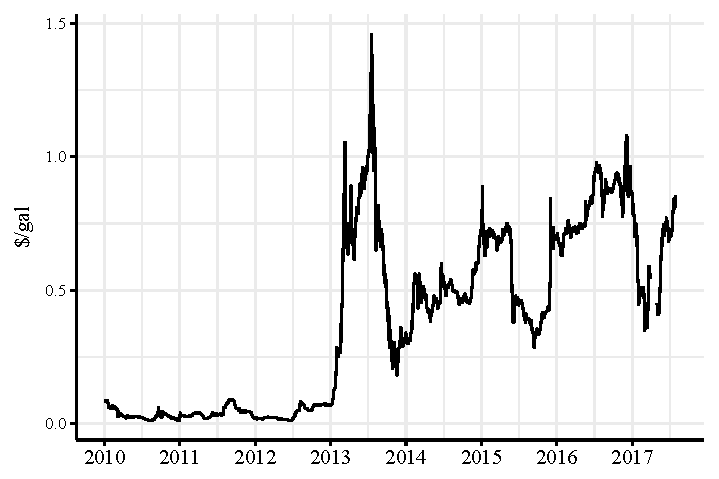
\includegraphics[width=\maxwidth]{figure/figure_rin-1} 

\end{knitrout}
\end{frame}

%%%%%%%%%%%%%%%%%%%%%%%%%%%%%%%%%%%%%%%%%%%%%%%%%%%%%%%%%%%%%%%%%%%%%%%%%%%%%%%%%%

\section{The blend wall}

\begin{frame}{Blend wall}
\begin{enumerate}[label=\textbullet]
    \item Currently, most ethanol is distributed through motor fuel that contains 10 percent ethanol (87-octane).
    \item This is the established maximum amount of ethanol in fuel that most engines can run on, without damage.
    \item Flex-fuel vehicles can run on fuel that contains more ethanol.
    \item In 2013, the mandate on ethanol blending slightly exceeded the blend wall for the blending of ethanol in regular 87-octane gasoline.
\end{enumerate}
\end{frame}

%%%%%%%%%%%%%%%%%%%%%%%%%%%%%%%%%%%%%%%%%%%%%%%%%%%%%%%%%%%%%%%%%%%%%%%%%%%%%%%%%%

\begin{frame}{Ethanol blend wall (up July 2017)}
\begin{knitrout}
\definecolor{shadecolor}{rgb}{0.969, 0.969, 0.969}\color{fgcolor}
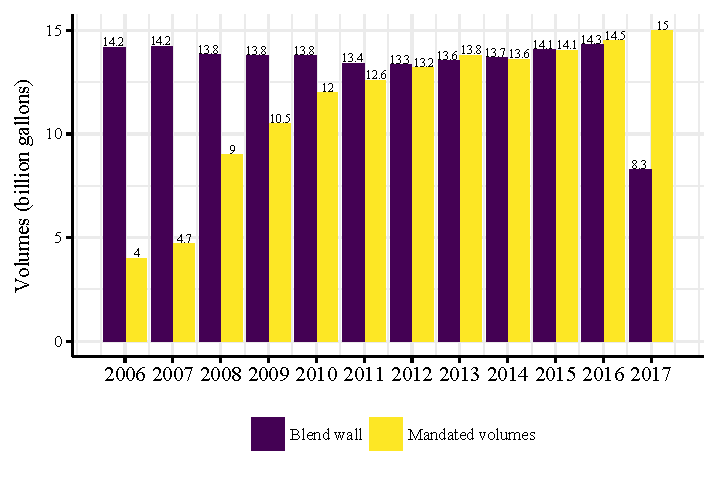
\includegraphics[width=\maxwidth]{figure/figure_wall-1} 

\end{knitrout}
\end{frame}

%%%%%%%%%%%%%%%%%%%%%%%%%%%%%%%%%%%%%%%%%%%%%%%%%%%%%%%%%%%%%%%%%%%%%%%%%%%%%%%%%%

\begin{frame}{Mandate vs production and consumption (up to May 2016)}
\begin{knitrout}
\definecolor{shadecolor}{rgb}{0.969, 0.969, 0.969}\color{fgcolor}
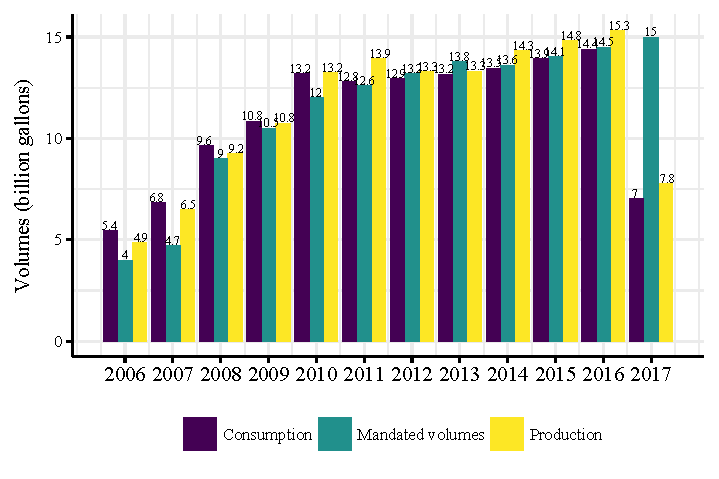
\includegraphics[width=\maxwidth]{figure/figure_rfs-1} 

\end{knitrout}
\scriptsize
\end{frame}

%%%%%%%%%%%%%%%%%%%%%%%%%%%%%%%%%%%%%%%%%%%%%%%%%%%%%%%%%%%%%%%%%%%%%%%%%%%%%%%%%%

\begin{frame}{2014 ethanol mandate}
\begin{enumerate}[label=\textbullet]
    \item In November 2013, EPA announced the ethanol mandate for 2014.
    \item EPA proposed an ethanol mandate for 2014 to 13 billion gallons, far short of the scheduled 14.4 billion gallons.
    \item The main reason that the EPA gave is that there was no distribution capacity for more ethanol.
    \item This was a very controversial decision:
      \begin{enumerate}[label=-]
          \item Farms and the ethanol industry voiced strong objections to the proposed rule. To them, more ethanol means more money;
          \item The oil industry was very happy with the proposed rule as the burden of meeting the ethanol mandate falls to them.
      \end{enumerate}
\end{enumerate}
\end{frame}

%%%%%%%%%%%%%%%%%%%%%%%%%%%%%%%%%%%%%%%%%%%%%%%%%%%%%%%%%%%%%%%%%%%%%%%%%%%%%%%%%%

\begin{frame}{2014 ethanol mandate -  oil industry argument}
\begin{enumerate}[label=\textbullet]
    \item In 2013, the oil industry, in particular the American Petroleum Insitute (API), organized a strong lobby for the EPA to reduce the ethanol mandate for 2014.
    \item The oil industry correctly pointed out that with a larger ethanol mandate, the price of RIN increases.
    \item The oil industry then claimed that this increase in cost would be passed to consumers, who would then decrease their consumption, which would make meeting the mandate more difficult.
    \item If the mandate keeps on increasing every year, the price of gasoline keeps on increasing, putting a significant dent on US economic growth.
    \item API even predicted that this will result in another recession.
\end{enumerate}
\end{frame}

%%%%%%%%%%%%%%%%%%%%%%%%%%%%%%%%%%%%%%%%%%%%%%%%%%%%%%%%%%%%%%%%%%%%%%%%%%%%%%%%%%

\begin{frame}{2014 ethanol mandate -  oil industry argument}
\begin{enumerate}[label=\textbullet]
    \item Were the arguments of the oil industry correct?
    \item Let's calculate the impact on the price of gasoline of a price of RIN \$1 per gallon of ethanol:
      \begin{enumerate}[label=-]
          \item Currently, the ethanol mandate requires blenders to acquire about 0.1 RIN for every gallon of gasoline;
          \item This means that the purchase of a RIN for each gallon of gasoline increases the cost of gasoline by 0.1 x \$1 = \$0.1 per gallon of gasoline;
          \item With a wholesale price of gasoline of about \$1.50 per gallon, this means that the cost of RIN increases wholesale gasoline by \$0.1 per gallon, or by about 6.7\%.
          \item The retail price of gasoline would also increase by about \$0.1 per gallon.
      \end{enumerate}
    \item Thus, a small increase in cost would result in a small change in consumption because the demand for gasoline is inelastic.
\end{enumerate}
\end{frame}

%%%%%%%%%%%%%%%%%%%%%%%%%%%%%%%%%%%%%%%%%%%%%%%%%%%%%%%%%%%%%%%%%%%%%%%%%%%%%%%%%%

\begin{frame}{2014 ethanol mandate -  oil industry argument}
\begin{enumerate}[label=\textbullet]
    \item At first glance, increasing the ethanol mandate would cause a small increase in gasoline price.
    \item I show with a colleague in a paper available \href{http://www.card.iastate.edu/policy_briefs/display.aspx?id=1218}{here} that the ethanol mandate might even cause a small decline in the price of gasoline.
    \item Our argument is that as the mandate increases, the value of ethanol going in gasoline will go down. This means that the price of motor fuel that contain a large share of ethanol (E85) will go down.
    \item E85 and E10 (regular gasoline), are substitute products.
    \item Thus, as more consumers purchase E85, the demand for gasoline shifts down, thus causing a decline in the price of gasoline at retail.
    \item That is, we find that the increase in the cost of producing gasoline is offset by substitution with other fuel blend.
\end{enumerate}
\end{frame}

%%%%%%%%%%%%%%%%%%%%%%%%%%%%%%%%%%%%%%%%%%%%%%%%%%%%%%%%%%%%%%%%%%%%%%%%%%%%%%%%%%

\begin{frame}{How to get over the blend wall?}
\begin{enumerate}[label=\textbullet]
    \item At the current volumes, it is possible to increase the ethanol mandate. However, US car fleet cannot accommodate much ethanol beyond the blend wall currently.
    \item There are many possible solutions to the blend wall:
    \begin{enumerate}[label=-]
        \item The EPA can modify the ethanol mandates;
        \item Other types of biofuel can be used to meet the mandate.
        \item Distribute ethanol through blends that contain more than 10 percent ethanol (e.g. E85). Is there really a demand for E85?
    \end{enumerate}
\end{enumerate}
\end{frame}

%%%%%%%%%%%%%%%%%%%%%%%%%%%%%%%%%%%%%%%%%%%%%%%%%%%%%%%%%%%%%%%%%%%%%%%%%%%%%%%%%%

\begin{frame}{How to get over the blend wall?}
\begin{enumerate}[label=\textbullet]
    \item Out of about 245 million vehicles, about 20 million can fuel with gasoline that contain more than 10 percent ethanol (flex vehicles).
    \item Out of about 110,000 fuel stations, less than 5 percent of them offer E85.
    \item The distribution capacity is a more limiting factor than the number of flex vehicles in increases sales of E85.
    \item Fuel stations do not have an incentive to increase their offering of E85 if the ethanol mandate does not increase.
    \item EPA did not increase the mandate because there was not enough distribution capacity for ethanol.
    \item This is a chicken and egg problem.
    \item I discuss this in a policy paper in more detail \href{http://www.card.iastate.edu/ag_policy_review/display.aspx?id=10}{here}.
\end{enumerate}
\end{frame}


%%%%%%%%%%%%%%%%%%%%%%%%%%%%%%%%%%%%%%%%%%%%%%%%%%%%%%%%%%%%%%%%%%%%%%%%%%%%%%%%%%

\begin{frame}{Is the future of US ethanol policy dead?}
\begin{enumerate}[label=\textbullet]
    \item EPA finally released the final rule for the 2014 ethanol mandates in June 2015.
    \item At the same time, EPA released mandates for 2015 and 2016.
    \item The mandate volumes are shown on slide \ref{slide.mandates}.
    \item EPA took a conservative approach by lowering the mandates but setting an increase in the mandates for the upcoming years.
    \item Those mandated volumes were much smaller than those that were scheduled.
\end{enumerate}
\end{frame}

%%%%%%%%%%%%%%%%%%%%%%%%%%%%%%%%%%%%%%%%%%%%%%%%%%%%%%%%%%%%%%%%%%%%%%%%%%%%%%%%%%

\section{Conclusions}

\begin{frame}{Conclusions}
\begin{enumerate}[label=\textbullet]
    \item US biofuel policy has an important impact on US energy supply and on US agriculture.
    \item Corn crop will influence the price of RINs.
    \item Current controversy regarding biodiesel.
\end{enumerate}
\end{frame}


%%%%%%%%%%%%%%%%%%%%%%%%%%%%%%%%%%%%%%%%%%%%%%%%%%%%%%%%%%%%%%%%%%%%%%%%%%%%%%%%%%%%
\section[References]{References}
\renewcommand\refname{References}
\def\newblock{References}
\begin{frame}{References}%[allowframebreaks]
\bibliography{D:/Dropbox/Papers/References}
%\bibliography{R:/users/pouliot/Papers/References}
%\bibliography{C:/Users/pouliot/Documents/Papers/References}
\end{frame}


%%%%%%%%%%%%%%%%%%%%%%%%%%%%%%%%%%%%%%%%%%%%%%%%%%%%%%%%%%%%%%%%%%%%%%%%%%%%%%%%%%%%%

\end{document}

